\documentclass{article}

% Configurações Genéricas ------------------------------------------------------
\usepackage[utf8]{inputenc}
\usepackage[T1]{fontenc}
\usepackage[brazil]{babel}
\usepackage{sbc-template}
\usepackage{graphicx}

% Informações Pessoais ---------------------------------------------------------
\title{Tarefa 03 sobre Desenvolvimento com Android}
\author{Wanderson Henrique Camargo Rosa\inst{1}}
\address{Programação para Dispositivos Móveis 2011/1\\Centro de Ciências Exatas
e Tecnológicas\\Universidade do Vale do Rio dos Sinos ---
UNISINOS\email{wandersonwhcr@gmail.com}}

% Documento --------------------------------------------------------------------
\begin{document}

\maketitle{}

% Introdução -------------------------------------------------------------------
\section{Introdução}
\label{sec:introducao}

O presente documento é resultado da terceira tarefa sobre desenvolvimento em
dispositivos móveis. Há a necessidade de criação de um programa simples e
funcional para o Sistema Operacional Android, porém não tão básico quanto os
fornecidos na documentação oficial da plataforma.

A Seção \ref{sec:ambiente} fala sobre como foi a instalação do ambiente de
desenvolvimento para Android utilizando Eclipse. Já a Seção \ref{sec:sobre}
descreve funcionalidades que o aplicativo deve possuir e a Seção
\ref{sec:presenter} dialoga sobre o primeiro projeto desenvolvido. Ao final, a
Seção \ref{sec:anotacoes} informa algumas anotações sobre o trabalho e quais são
as próximas funcionalidades que deverão ser incluídas.

% Instalação do Ambiente -------------------------------------------------------
\section{Instalação do Ambiente}
\label{sec:ambiente}

Utilizando o ambiente de desenvolvimento Eclipse, instalei os plugins
necessários para programação na plataforma com sucesso, inclusive com plena
execução sobre uma plataforma 64 bits, algo que gerou erros no desenvolvimento
em J2ME.

Existe um binário que é utilizado para comunicação entre o dispositivo móvel e a
máquina de desenvolvimento chamado Android Debug Bridge (ADB), que deve ser
anexado externamente ao ambiente. Como já tive alguma experiência em programação
com esta tecnologia, a instalação não gerou problemas.

Após criar um novo projeto, o próprio Eclipse gerou um erro informando que não
existiam todas as ferramentas necessárias. Isto aconteceu porque era preciso a
instalação das bibliotecas. Após adição da API 8 do Android 2.2 Froyo, nenhum
erro foi gerado. Para aprendizado da linguagem, implementei alguns programas de
exemplo disponíveis na documentação oficial e na disciplina.

% Sobre o Aplicativo -----------------------------------------------------------
\section{Sobre o Aplicativo}
\label{sec:sobre}

Conforme relatório anterior da segunda tarefa, será implementado um apresentador
de \emph{slides} para Android que estou idealizando há quase 1 ano.

Um apresentador de \emph{slides} é um dispositivo de hardware que permite o
controle das lâminas de apresentações, palestras ou seminários à distância, sem
a necessidade de deslocamento até a máquina onde os documentos estão sendo
exibidos, fazendo que o ministrante tenha uma melhor interação com o público.
Este dispositivo é relativamente caro em comparação com as funcionalidades
simples disponíveis. Porém, podemos construir um programa sobre a plataforma
Android que consegue suprir as mesmas necessidades.

A tarefa atual consiste em inicializar o desenvolvimento deste aplicativo,
criando uma comunicação simples entre dispositivo móvel e computador, utilizando
Bluetooth ou conexão por Sockets.

\subsection{Teoria de Aplicação}

Se criarmos um programa capaz de receber qualquer dado do dispositivo móvel
utilizando algum tipo de conexão, enviando estas informações para a saída
padrão, com certeza será possível a implementação do apresentador de
\emph{slides}.

\subsection{Serviço de Conexão}

Primeiramente era necessário criar um servidor simples capaz de receber conexões
por Sockets. Utilizando a linguagem de programação Java, criei um simples
programa que abre um serviço e aguarda uma conexão de um cliente.

Quando esta conexão é estabelecida, o servidor espera um número inteiro que
representa a quantidade de bytes que serão enviados. Após, recebe do cliente a
quantidade de bytes propriamente dita, exibindo estas informações na saída
padrão. Ao final da transferência a conexão é fechada. Estas regras representam
um primeiro protocolo básico para comunicação do aplicativo.

Para melhorar o estudo sobre a programação, criei uma máquina virtual de 32 bits
com um Sistema Operacional Debian Linux. Após, instalei a última versão da JRE
disponível nos repositórios do Debian. Após, criei um pacote JAR do servidor e
executei na máquina virtual.

Qualquer binário gerado deve ser executado da mesma maneira entre diferentes
Sistemas Operacionais que utilizam a JRE. Portanto, teoricamente, estes testes
também serão válidos entre outros SO em que a JRE seja executada.

% Presenter --------------------------------------------------------------------
\section{Presenter}
\label{sec:presenter}

O aplicativo Presenter v0.1 representa a primeira estrutura necessária para
conexão entre dispositivo móvel com Sistema Operacional Android e um serviço
qualquer utilizando Sockets, fruto da terceira tarefa desta disciplina. Existe
um pequeno protocolo de comunicação, onde primeiramente é enviado um número
representante da quantidade de bytes que devem ser enviados e, após, a
quantidade de bytes propriamente dita. Ao término do envio a conexão é fechada.

\subsection{Necessidades}

Há a necessidade de configurações sobre o servidor e porta para conexão. Estas
informações devem ser salvas em local apropriado para posterior acesso, evitando
a entrada dos dados sempre que este aplicativo seja utilizado.

O aplicativo deve possuir um campo para preenchimento da mensagem que será
enviada para o servidor e um botão de envio. Deve existir uma separação entre
tela principal para envio da mensagem e tela de configurações de servidor,
acessíveis através de um menu específico.

\subsection{Implementação}

O aplicativo trabalha sobre algumas funcionalidades do Android. A sua estrutura
pode ser visualizada conforme a Figura \ref{fig:project}. Existe uma tela
principal, que possui um campo para preenchimento de mensagem e um botão de
envio. Neste foi adicionado um menu de contexto com um único botão para acesso
às configurações.

\begin{figure}
    \centering{}
    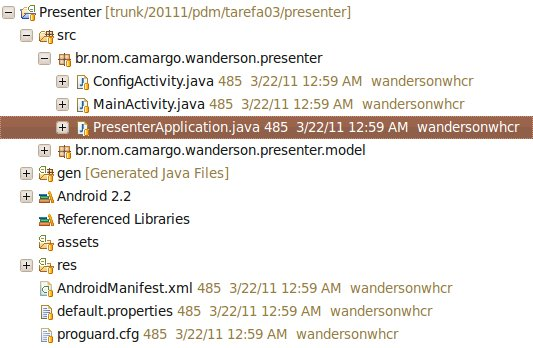
\includegraphics[scale=0.45]{screenshot01-project}
    \caption{Estrutura do Aplicativo}
    \label{fig:project}
\end{figure}

A tela de configurações possui um campo de texto que recebe o endereço de IP e
outro para a porta. Logo abaixo existe um botão para salvar os dados fornecidos.

\subsection{Banco de Dados}

Os valores das configurações são armazenadas em banco de dados SQLite fornecido
pelo próprio Android e armazenado em local específico. Para manipulação do banco
desenvolvi a classe \texttt{DatabaseHelper} estendida de
\texttt{SQLiteOpenHelper} que auxilia a instalação do banco e criação da única
tabela que armazena as configurações necessárias, inserindo os valores iniciais
para endereço de conexão no servidor e porta. Também foi adicionada uma camada
de modelo para a tabela de configurações, encapsulando o acesso a estes valores.

Buscando centralizar o acesso ao banco de dados, necessito da inclusão do padrão
de projeto Singleton que evita a criação de dois objetos desta classe. Ao
efetuar uma pesquisa mais aprofundada, descobri que existe uma classe
representante do aplicativo por completo e que pode ser utilizada como este
padrão.

\subsection{Aplicativo}

Como uma extensão da classe \texttt{Application} do Android, criei uma classe
local chamada \texttt{PresenterApplication} que recebe um objeto da classe
\texttt{DatabaseHelper} e métodos de acesso para centralizar o banco de dados.
Tive que alterar o arquivo \texttt{AndroidManifest.xml} para que esta classe
seja considerada como base do aplicativo.

\subsection{Atividades e Intenções}

Uma atividade é uma classe estendida de \texttt{Activity} que trabalha com a
interação entre usuário e Sistema Operacional. Neste aplicativo, ela representa
as telas disponíveis. Para comunicação entre as atividades são inicializadas as
intenções, representadas pela classe \texttt{Intent}.

O aplicativo possui duas telas, a atividade \texttt{MainActivity} que trabalha
como principal e recebe o campo de mensagem e botão de envio, conforme a Figura
\ref{fig:main}. Também há \texttt{ConfigActivity} que fornece os campos de
configuração, conforme a Figura \ref{fig:config}. Ambas são classes que estendem
de \texttt{Activity}.

\begin{figure}
    \centering{}
    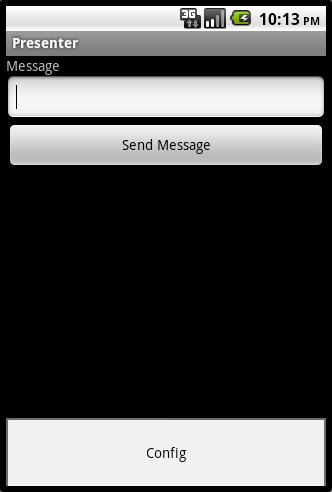
\includegraphics[scale=0.3]{screenshot02-main.jpg}
    \caption{Atividade Principal do Aplicativo}
    \label{fig:main}
\end{figure}

A tela principal envia uma intenção ao Sistema Operacional solicitando a tela de
configuração quando o botão do menu de contexto é pressionado. Quando a
atividade de configuração está sendo utilizada, o botão para salvar as
informações finaliza a tela. Esta, em tempo de finalização, salva as informações
através da camada de modelo.

\begin{figure}
    \centering{}
    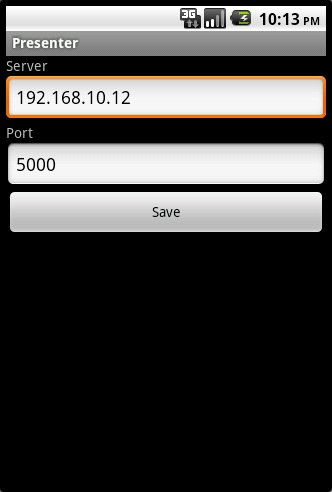
\includegraphics[scale=0.3]{screenshot03-config.jpg}
    \caption{Tela de Configurações}
    \label{fig:config}
\end{figure}

\subsection{Comunicação}

Toda a lógica de transferência de informações está descrita na classe
\texttt{MainActivity}. Quando o botão de envio é pressionado, um Socket é aberto
a partir das configurações de servidor e porta. O conteúdo do campo de
mensagem é transformado em um \emph{array} de bytes. Seguindo o protocolo,
primeiramente é enviada a quantidade de bytes que serão transmitidos e após os
bytes propriamente ditos. Ao final da transferência, a conexão é finalizada.

Quando os dados são enviados com sucesso, o usuário é informado do recebimento
correto através de uma mensagem flutuante. Se houve algum erro em tempo de
transferência, uma mensagem semelhante é exibida informando o ocorrido.

A comunicação somente foi aceita pelo Sistema Operacional após a inclusão da
regra de conexão à Internet no gerenciador de permissões do
\texttt{AndroidManifest.xml}. Caso contrário, uma exceção de acesso negado é
gerada.

\subsection{Execução}

A versão atual v0.1 foi testada no emulador disponível pelo ambiente de
desenvolvimento e no \emph{smartphone} Samsung Galaxy 5 com Android 2.2
Froyo, conforme a Figura \ref{fig:smart}. O aplicativo APK somente foi gerado
após a criação de uma \emph{keystore} solicitado pelo ambiente de
desenvolvimento. Por sua simplicidade, não gerou erros em tempo de execução, mas
por causa da conexão bloqueante por Sockets o celular travou em alguns momentos.

\begin{figure}
    \centering{}
    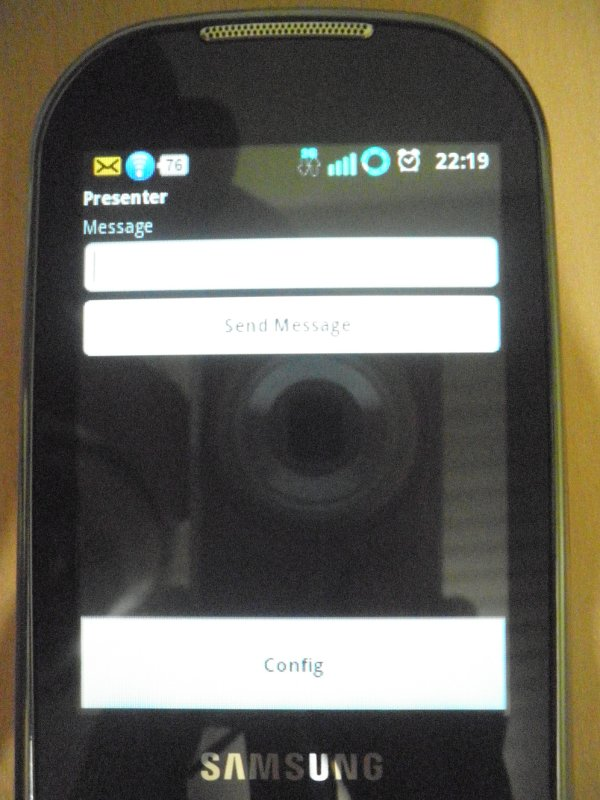
\includegraphics[scale=0.3]{screenshot04-smart.jpg}
    \caption{Aplicativo Executando sobre um \emph{Smartphone}}
    \label{fig:smart}
\end{figure}

% Anotações Finais -------------------------------------------------------------
\section{Anotações Finais}
\label{sec:anotacoes}

Em uma primeira análise, o desenvolvimento com o Sistema Operacional Android
parece um pouco confuso porque existe uma estrutura de diretórios muito rígida.
Porém ao compreendê-la, consegui trabalhar tranquilamente sobre a plataforma,
inclusive porque a linguagem de programação utilizada é Java.

Há algum tempo eu tentei programar alguns aplicativos para este SO mas encontrei
problemas quando era necessária a criação de \emph{layouts}. Hoje o ambiente de
desenvolvimento possui uma \emph{interface} para construção que me auxiliou
muito, sendo muito fiel ao ambiente real de execução.

Não foram incluídos tratamentos ou refinamentos da entrada de dados pelo usuário
nesta versão, nem ícones para melhor identificação das funcionalidades
acessadas. O aplicativo atual executa a comunicação sobre o fluxo principal de
execução, bloqueando o usuário até que todas as informações sejam transferidas.
Isto é facilmente corrigido com a separação desta funcionalidade em uma
\emph{thread} secundária.

Para instalação do ambiente e programação do primeiro projeto disponível na
documentação foram gastas 2h. A criação do servidor de conexão para testes,
incluindo instalação do Sistema Operacional e desenvolvimento, foi executada em
1h30min. A conexão por sockets em um ambiente de tela única foi finalizada em
3h30min e a inclusão de uma tela secundária com acesso ao banco de dados
executou-se em 4h. A documentação final foi escrita em cerca de 4h. Ao total, o
desenvolvimento deste aplicativo levou 15h distribuidas entre os dias 15 de
março e 22 de março de 2011.

\subsection{Continuidade do Projeto}

Em um segundo momento, na quarta tarefa desta disciplina, pretendo continuar com
o desenvolvimento deste aplicativo, incluindo as funcionalidades discutidas
nesta Seção. O protocolo será modificado e o servidor irá receber informações
sobre navegação. A tela do cliente irá trabalhar com botões para navegação,
transferindo as informações utilizando Bluetooth.

\end{document}